\subsection{About the Hardware}
% \addcontentsline{toc}{section}{About the Hardware}

    \paragraph*{}
    The performance of a CPU (Central Processing Unit) depends on more than just its raw processing power. 
    Both its architecture—how it’s designed and organized—and the surrounding hardware play critical roles in 
    its overall efficiency. Components such as memory or storage interact closely with the CPU, influencing how well 
    it handles tasks. Additionally, understanding key concepts related to CPU architecture, like cores, threads, and cache, 
    is essential for grasping the full picture of system performance. 
    \par

    \vspace{-1em}

    \paragraph*{}
    In this section, we will explore both the architectural aspects of the CPU and the related hardware that together 
    drive the performance of modern computing systems.
    \par



\subsubsection{How CPU works}
% \addcontentsline{toc}{subsection}{How CPU works}

    \paragraph*{}
    The CPU operates by \textbf{fetching} instructions and data from memory, which it \textbf{processes} using its registers—small, 
    fast storage locations within the CPU. These registers temporarily hold data and instructions during processing, 
    allowing the CPU to quickly access and manipulate information. The CPU uses a cycle of \textbf{fetch, decode, and execute} 
    to perform operations, where it retrieves the necessary data from memory, decodes the instructions, and then executes 
    them using the registers for efficient data handling.
    \par

    \paragraph*{}
    It is important to distinguish between the functioning at the thread level and the core level. 
    A CPU core typically has two threads, allowing it to handle multiple instructions concurrently through 
    simultaneous multithreading (SMT). While each thread functions independently, sharing resources such as 
    registers and execution units within the core, the overall performance and efficiency of the CPU are significantly 
    influenced by how these threads interact and share the core’s resources. The ability to manage tasks at both the 
    core and thread levels is crucial for optimizing CPU performance, particularly in parallel computing environments.
    \par


\subsubsection{Micro-operations and pipelining}
% \addcontentsline{toc}{subsection}{Micro-operations and pipelining}

    \paragraph*{Micro-operations} 
    Micro-operations, are the smaller instructions into which complex CPU
    instructions are broken down. Modern CPUs often deal with complex instructions that are not directly 
    executable by the CPU’s hardware. To manage this complexity, these instructions are divided into simpler 
    operations known as micro-operations. The CPU can then execute them more efficiently using its execution units.
    \par
    
    \paragraph*{Pipelining} 
    Pipelining is a technique used in CPUs to improve instruction throughput—the number of 
    instructions that can be processed in a unit of time. In a pipelined CPU, a single instruction is broken down into multiple 
    stages (like fetching, decoding, executing, etc.), and these stages are processed in parallel for different instructions. 
    However, this doesn't mean that different threads are assigned specific stages like fetch or decode. Instead: one thread can go 
    through all the stages of the pipeline for different instructions over time. For example, while one instruction is being 
    executed, the next instruction might be in the decode stage, and yet another instruction might be in the fetch stage, all 
    within the same thread and the same pipeline.
    \par



\subsubsection{Vectorization: AVX}
% \addcontentsline{toc}{subsection}{AVX512, FMA}

    \paragraph*{}
    Vectorization is the process of transforming operations that are performed sequentially (one by one) into operations that can be 
    performed simultaneously on multiple data points. This is achieved by processing "vectors" of data instead of processing a single 
    value at a time.
    \par

    \paragraph*{}
    For example, instead of adding two numbers at a time, a processor with vectorization can add several numbers simultaneously using 
    a single instruction. This is known as SIMD (Single Instruction, Multiple Data), meaning one instruction operates on multiple data 
    points in parallel.
    \par

    \paragraph*{}
    AVX-512 is a technology that implements and enhances vectorization in CPUs. It works through SIMD instructions and introduces larger registers 
    (512 bits) that allow more data to be handled at once in a single operation. For example, instead of performing an addition 
    on just two numbers, AVX-512 can process 16 numbers of 32 bits or 8 numbers of 64 bits at the same time.
    \\
    In addition to AVX-512, processors typically include AVX or AVX2, both of which feature 256-bit registers, half the size of 
    AVX-512 registers. To check if your processor supports AVX, AVX2, or AVX-512, you can run the following Julia code to display 
    your processor’s specifications:
    \\
    \begin{lstlisting}[language=Julia]
        Pkg.add("CpuId")
        using CpuId

        # View all processor features
        cpuid = cpuinfo()
    \end{lstlisting}
    \vspace{0.5cm}
    
    In your terminal, you will be able to see whether your registers are 256 bits (indicating AVX or AVX2) or 512 bits 
    (indicating AVX-512). Additionally, if you are working from a laptop, you may also notice a Turbo Boost value, which 
    refers to a different GHz value. This is the value that will be used in future theoretical calculations.

    

    \subsubsection{Memory: RAM}

    \paragraph*{}
    Random Access Memory (RAM) is a type of volatile memory that temporarily stores data and instructions needed 
    by the CPU to perform tasks. RAM typically stores data in the order of gigabytes (GB), allowing the system 
    to manage multiple active programs and processes simultaneously. This supports the smooth execution of complex 
    operations.
    \par

    \paragraph*{}
    However, RAM speed is slower than CPU speed, which can lead to bottlenecks. In such cases, the performance of 
    the CPU is limited by the data transfer speed from the RAM. Some examples of RAM data transmission times, 
    taken from the document [...], are:
    \begin{enumerate}
        \item Memory 3200 MHz, CL16: $\frac{16}{3200} \times 1000 \simeq 5 [ms]$
        \item Memory 4000 MHz, CL19: $\frac{19}{4000} \times 1000 \simeq 4.75 [ms]$
        \item  Memory 2400 MHz, CL17: $\frac{17}{2400} \times 1000 \simeq 7.08 [ms]$
    \end{enumerate}
    
    
   
\subsubsection{Memory: Cache}
% \addcontentsline{toc}{subsection}{Memory}

    \paragraph*{}
    In modern computing, the CPU is tasked with processing vast amounts of data and instructions at incredible speeds. 
    However, retrieving this information from the main memory (RAM) can be relatively slow, creating a bottleneck that 
    limits the CPU's performance. To bridge this gap and ensure the CPU can work as efficiently as possible, cache 
    memory was introduced. Cache serves as a high-speed storage located closer to the CPU, designed to temporarily 
    hold frequently accessed data and instructions. This reduces the time the CPU spends waiting for data retrieval, 
    significantly improving system performance.
    \par

    \paragraph*{}
    Modern CPUs use a multi-level cache hierarchy to enhance performance. Typically, there are three levels: L1, L2, 
    and L3. L1 cache is the smallest but fastest and resides directly within the CPU cores. L2 cache is larger and 
    slightly slower, while L3 is even bigger but still significantly faster than RAM. By utilizing these cache 
    levels, CPUs can prioritize faster access to data that is more likely to be used again. The efficiency of 
    this system ensures that the CPU spends less time waiting for data retrieval and more time processing information.
    \par

    \paragraph*{}
    The following diagram illustrates the different levels of memory in a typical computer system, arranged in a pyramid to 
    highlight the trade-offs between speed, cost, and capacity. At the top, CPU registers and cache memory (SRAM) 
    are the fastest and most expensive per bit, but offer limited capacity. As we move down the pyramid, memory types 
    like main memory (DRAM) and storage solutions such as magnetic disks and optical disks provide larger capacities 
    but come with slower access times and lower costs per bit. This hierarchy demonstrates the balance between speed 
    and storage, emphasizing why cache memory plays such a crucial role in optimizing CPU performance by acting as 
    an intermediary between the extremely fast CPU registers and the slower but more abundant main memory and storage.

    \begin{figure}[h]
        \begin{center}
            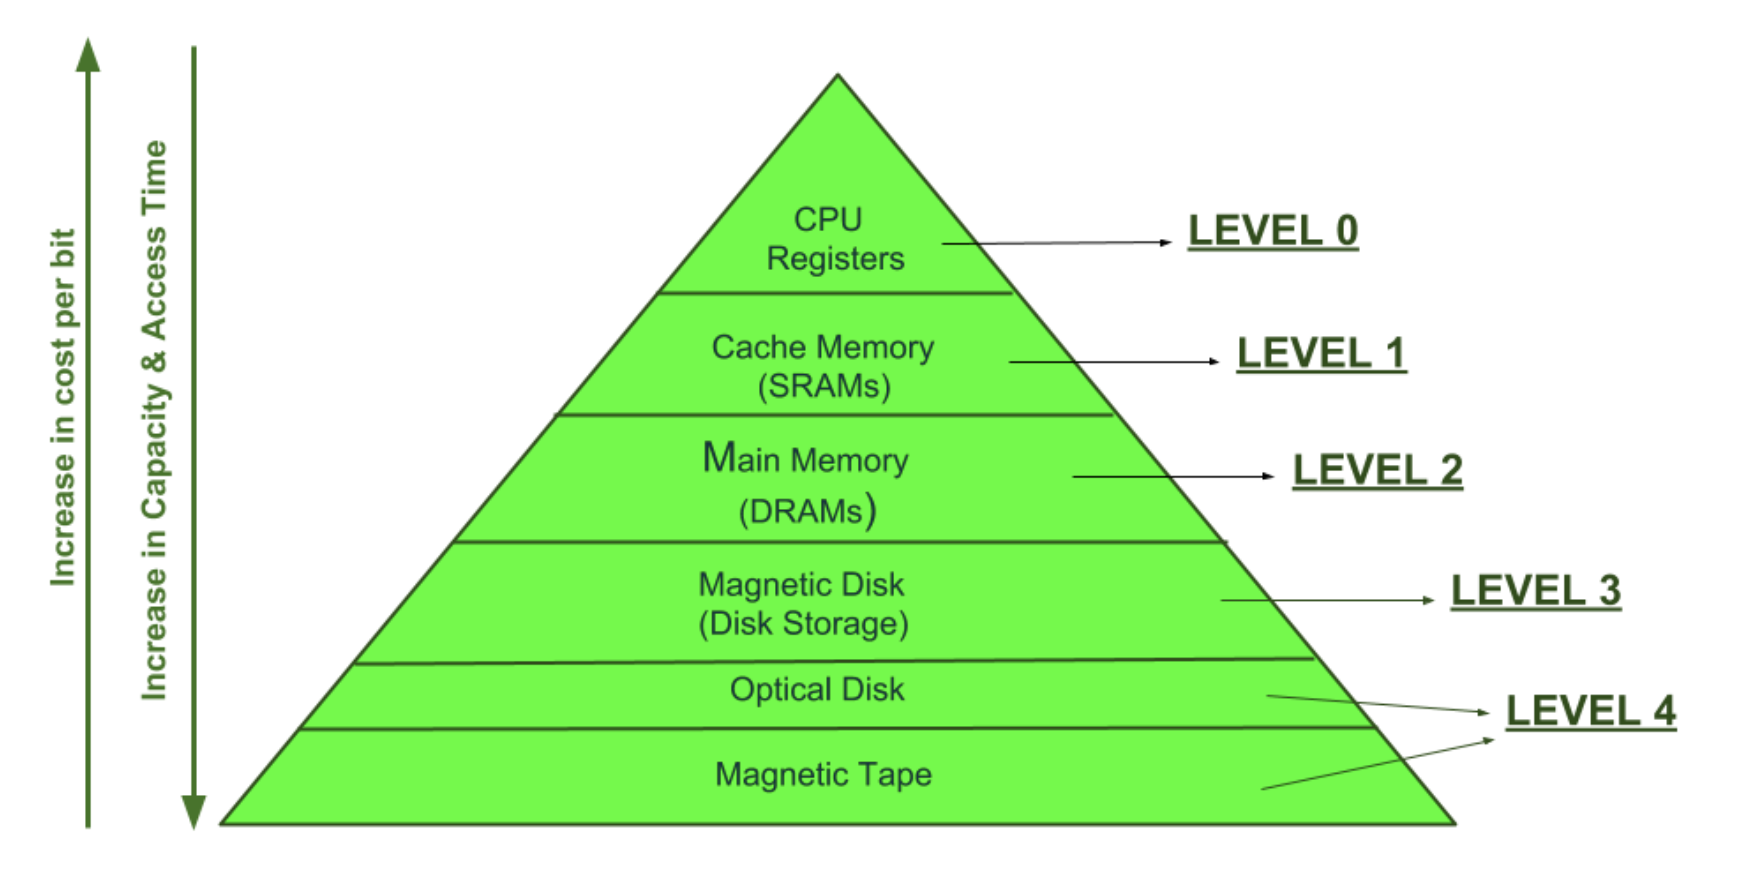
\includegraphics[width=0.6\textwidth]{Figures/herarchy.png}
        \end{center}
        \caption{Representation of the hierarchy of different types of memory in a system.}
        \label{}
    \end{figure}

\newpage